\documentclass{article}
\usepackage{tikz}
\usepackage{geometry}
\geometry{a4paper, margin=1in}
\usepackage{everypage}
\usepackage{amsmath}
\usepackage{amssymb}
\usepackage{algorithm}
\usepackage{algpseudocode}
\usepackage{listings}
\usepackage{xcolor}
\usepackage{enumitem}
\usepackage{xepersian}
\settextfont{Vazirmatn}
\usetikzlibrary{calc}


\definecolor{codegreen}{rgb}{0,0.6,0}
\definecolor{codegray}{rgb}{0.5,0.5,0.5}
\definecolor{codepurple}{rgb}{0.58,0,0.82}
\definecolor{backcolour}{rgb}{0.97,0.97,0.95}

\lstdefinestyle{pythonstyle}{
    backgroundcolor=\color{backcolour},   
    commentstyle=\color{codegreen},
    keywordstyle=\color{codepurple},
    numberstyle=\tiny\color{codegray},
    stringstyle=\color{orange},
    basicstyle=\ttfamily\small,
    breakatwhitespace=false,         
    breaklines=true,                 
    captionpos=b,                    
    keepspaces=true,                 
    numbers=left,                    
    numbersep=5pt,                  
    showspaces=false,                
    showstringspaces=false,
    showtabs=false,                  
    tabsize=2,
    frame=single
}
\lstset{style=pythonstyle}

\AddEverypageHook{
\begin{tikzpicture}[remember picture,overlay]
\draw[line width=1pt]
    ($(current page.north west)+(1cm,-1cm)$)
    rectangle
    ($(current page.south east)+(-1cm,1cm)$);
\end{tikzpicture}
}

\begin{document}
\begin{titlepage}
\centering

به نام خدا\\

\includegraphics[width=0.3\textwidth]{image.png}\\
\vspace{0.4cm}
پروژه درس جبر خطی – ترم 4042\\
\vspace{1.5cm}
\textbf{\Large Latent Semantic Indexing}\\
\vspace{0.4cm}
استاد : دکتر نیکان\\
\vspace{0.4cm}
اعضای گروه: علی کارخانه  - مصطفی شیبانی – حسین نادری – مرتضی رحیمی
\end{titlepage}

\section*{سوالات عملی:}


\textbf{سوال ۷ --- بارگذاری و پیش‌پردازش متن (حذف علائم نگارشی و کوچک‌سازی حروف)}
    
\noindent در پروژه‌های بازیابی اطلاعات و نمایه سازی پنهان متن ،(LSI) پیش‌پردازش متن یکی از حیاتی‌ترین مراحل است. هدف از این کار، حذف اطلاعات بیهوده (Noise) و یکدست‌سازی کلمات است تا محاسبات برداری دقیق‌تر انجام شوند. کد زیر فرآیند تمیزکاری متون را انجام می‌دهد:

\begin{latin}

\begin{lstlisting}[language=Python]
# ============================================================
# Q7 — Load + preprocess (lowercase, remove punctuation)
# ============================================================
def preprocess(text):
    text = text.lower()
    text = re.sub(r'[^a-z\s]', ' ', text)
    text = re.sub(r'\s+', ' ', text).strip()
    return text

def q7_load_and_preprocess():
    df = pd.read_csv(DATA_PATH)
    print("Q7 | Dataset shape:", df.shape)
    df['clean_text'] = df['Text'].apply(preprocess)
    return df
\end{lstlisting}
\end{latin}
    \subsection*{توضیح عملکرد متدها و توابع:}

    \paragraph{۱. تابع \texttt{preprocess(text)}:}\hspace{-10pt}
    این تابع یک متن خام را به عنوان ورودی دریافت کرده و مراحل زیر را روی آن اعمال می‌کند تا متنی یکدست ایجاد شود:
    \begin{itemize}
        \item \textbf{تبدیل به حروف کوچک ( text.lower() )}: 
        تمام حروف بزرگ انگلیسی به حروف کوچک تبدیل می‌شوند. این کار باعث می‌شود کلماتی مانند \lr{``Data''} و \lr{``data''} یکسان دیده شوند و ابعاد ماتریس نهایی بیهوده بزرگ نشود.
        
        \item \textbf{حذف کاراکترهای غیرالفبایی} : 
        با استفاده از عبارات منظم ( Regular Expressions )، هر کاراکتری که جزء حروف الفبای انگلیسی (\lr{a-z}) یا فاصله (\lr{\textbackslash{}s}) نباشد، با یک فاصله معمولی جایگزین می‌شود. این کار علائم نگارشی نظیر ویرگول، نقطه، علامت سوال و همچنین اعداد را کاملاً حذف می‌کند.
        
        \item \textbf{حذف فاصله‌های اضافه}: 
        حذف علائم نگارشی در مرحله قبل ممکن است چندین فاصله متوالی ایجاد کرده باشد. الگوی \lr{\textbackslash{}s+} تمام فاصله‌های متوالی را به یک تک‌فاصله تبدیل می‌کند و متد \texttt{.strip()} نیز فاصله‌های خالی ابتدا و انتهای متن را پاک می‌کند.
    \end{itemize}

    \paragraph{۲. تابع \texttt{q7\_load\_and\_preprocess()}:}\hspace{-10pt}
    این تابع وظیفه مدیریت جریان داده را بر عهده دارد:
    \begin{itemize}
        \item ابتدا مجموعه داده را از مسیر \texttt{DATA\_PATH} به صورت یک دیتافریم پانداس بارگذاری می‌کند.
        \item با چاپ \texttt{df.shape}، ابعاد داده‌ها (تعداد کل اسناد و ویژگی‌ها) را جهت بررسی صحت بارگذاری نمایش می‌دهد.
        \item در نهایت با استفاده از متد \texttt{.apply()}، تابع تمیزکاری متنی را روی تک‌تک سطرهای ستون \texttt{'Text'} اعمال کرده و نتیجه را در ستون جدیدی به نام \texttt{'clean\_text'} ذخیره می‌کند.
    \end{itemize}

    \paragraph{۳. خروجی اجرای تابع و تحلیل ساختار داده‌ها:}\hspace{-10pt}
    پس از فراخوانی تابع بارگذاری و پیش‌پردازش متنی، پیش‌نمایشی از دیتافریم خروجی به همراه ابعاد آن تولید می‌شود:

    \begin{figure}[h!]
        \centering
        % نام فایل تصویر خود را در بخش زیر جایگزین کنید (مثلاً q7_output.png)
        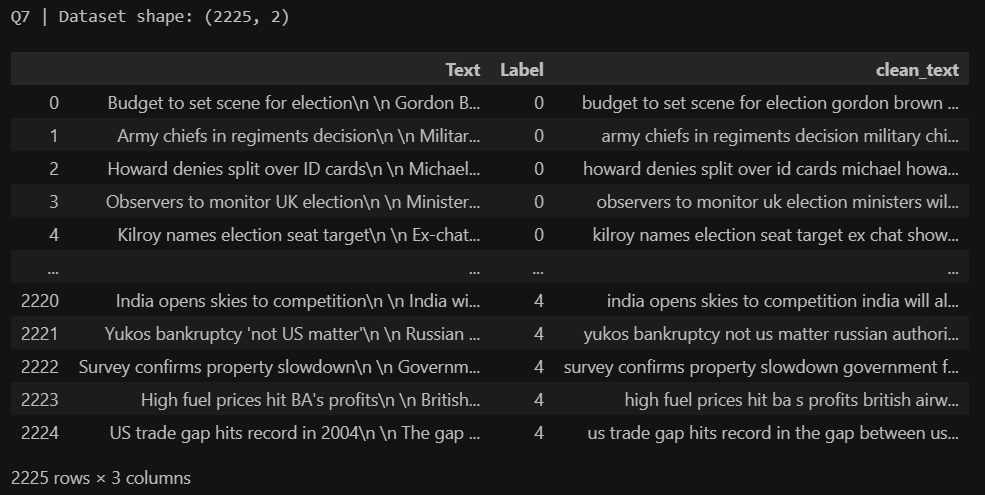
\includegraphics[width=0.9\textwidth]{Output7.png} 
        \caption{خروجی نهایی دیتافریم پس از انجام عملیات پیش‌پردازش متنی}
        \label{fig:q7_output}
    \end{figure}

    \begin{itemize}
        \item \textbf{ابعاد مجموعه داده (\lr{Dataset shape: (2225, 2)}):} 
        خروجی نشان می‌دهد که دیتاست اولیه دارای ۲۲۲۵ سطر (سند متنی) و ۲ ستون اصلی است. پس از اجرای تابع و اضافه شدن ستون تمیزشده، تعداد ستون‌ها به ۳ افزایش می‌یابد (\lr{2225 rows $\times$ 3 columns}).
        
        \item \textbf{بررسی ساختار ستون‌ها:}
        \begin{enumerate}
            \item \textbf{ستون \texttt{Text}:} شامل متن خام اسناد است که در آن علائم نگارشی، کاراکترهای خط جدید (\lr{\textbackslash{}n}) و حروف بزرگ انگلیسی به همان شکل اولیه دیده می‌شوند.
            \item \textbf{ستون \texttt{Label}:} شامل برچسب‌های عددی (مثلاً دسته $0$ برای سیاست و دسته $4$ برای تجارت) است که دسته‌بندی موضوعی اسناد را مشخص می‌کند.
            \item \textbf{ستون جدید \texttt{clean\_text}:} خروجی نهایی حاصل از اعمال تابع \lr{\texttt{preprocess}} است. همان‌طور که در تصویر مشخص است، تمامی حروف بزرگ به حروف کوچک تبدیل شده‌اند، کاراکترهای کنترلی مانند \lr{\textbackslash{}n} و علائم نگارشی کاملاً حذف شده و کلمات صرفاً با یک تک‌فاصله از یکدیگر جدا شده‌اند تا برای پردازش‌های بعدی آماده باشند.
        \end{enumerate}
    \end{itemize}
\noindent\textbf{سوال ۸ --- استخراج ۳۰ کلمه پرتکرار و رسم نمودار میله‌ای }
    
\noindent در این بخش، هدف شناسایی و استخراج ۳۰ کلمه پرتکرار موجود در کل اسناد با امکان فعال یا غیرفعال‌سازی فیلتر کلمات توقف (\lr{Stopwords}) است. کد مربوط به این بخش به صورت زیر است:

\begin{latin}
\begin{lstlisting}[language=Python]
# ============================================================
# Q8 — Top 30 most frequent words + bar chart
# ============================================================
def q8_top30_words(df, fname, stopwords=False):
    if stopwords:
        stopwords = ENGLISH_STOP_WORDS
    else:
        stopwords = {}
        
    stop_words_set = set(stopwords)

    all_words = []
    for text in df['clean_text']:
        words = [w for w in text.split() if w not in stop_words_set and len(w) > 1]
        all_words.extend(words)

    counter = Counter(all_words)
    top30 = counter.most_common(30)
    print("\nQ8 | Top 30 frequent words:", top30)

    words, counts = zip(*top30)
    fig, ax = plt.subplots(figsize=(14, 6))
    ax.bar(words, counts, color='steelblue')
    plt.xticks(rotation=60, ha='right')
    ax.set_title('Top 30 Most Frequent Words (all documents)')
    ax.set_ylabel('Frequency')
    plt.tight_layout()
    % plt.savefig(f'media/{fname}.png', dpi=130)
    plt.close(fig)
    
    return top30
\end{lstlisting}
\end{latin}

    \subsection*{توضیح عملکرد متدها و توابع:}

    \paragraph{۱. منطق شرطی کلمات توقف (\texttt{stopwords} و \texttt{stop\_words\_set}):}\hspace{-10pt}
    تابع در این نسخه منعطف‌تر طراحی شده است و پارامتر \lr{\texttt{stopwords}} را به عنوان ورودی می‌پذیرد:
    \begin{itemize}
        \item اگر مقدار \lr{\texttt{stopwords}} برابر با \lr{\texttt{True}} پاس داده شود، کلمات توقف استاندارد انگلیسی (\lr{\texttt{ENGLISH\_STOP\_WORDS}}) به عنوان فیلتر فعال می‌شوند.
        \item در غیر این صورت (حالت \lr{\texttt{False}})، یک دیکشنری خالی \lr{\texttt{\{\}}} تخصیص داده می‌شود که به معنی عدم فیلتر کردن کلمات توقف است.
        \item کلمات توقف در نهایت به یک ساختار مجموعه (\lr{\texttt{set}}) تبدیل می‌شوند؛ زیرا جستجو در ساختار مجموعه در پایتون از مرتبه زمانی $O(1)$ بوده و سرعت پردازش را بسیار افزایش می‌دهد.
    \end{itemize}

    \paragraph{۲. جمع‌آوری و فیلتر کلمات:}
    \begin{itemize}
        \item با پیمایش ستون متون تمیزشده (\lr{\texttt{clean\_text}})، هر متن با متد \texttt{.split()} به کلمات سازنده‌اش شکسته می‌شود.
        \item کلماتی که در مجموعه‌ی کلمات توقف تعریف‌شده وجود نداشته باشند (\lr{\texttt{w not in stop\_words\_set}}) و طول آن‌ها بزرگتر از یک حرف باشد (\lr{\texttt{len(w) > 1}})، فیلتر شده و به لیست نهایی اضافه می‌گردند.
    \end{itemize}

    \paragraph{۳. شمارش و استخراج ۳۰ کلمه برتر:}\hspace{-10pt}
    کلاس \lr{\texttt{Counter}} فرکانس تکرار کلمات را محاسبه کرده و با متد \lr{\texttt{most\_common(30)}}، ۳۰ کلمه با بیشترین تکرار را به صورت لیستی از توپل‌های (کلمه, فرکانس) باز می‌گرداند.

    \paragraph{۴. رسم و مدیریت نمودار میله‌ای:}
    \begin{itemize}
        \item با دستور \lr{\texttt{zip(*top30)}} داده‌ها باز شده و به دو بخش کلمات و فرکانس‌ها تقسیم می‌شوند تا در نمودار میله‌ای به کار روند.
        \item نمودار میله‌ای با رنگ آبی فولادی (\lr{\texttt{steelblue}}) رسم شده و برچسب‌های محور افقی جهت جلوگیری از هم‌پوشانی ۶۰ درجه چرخانده می‌شوند.
        \item نام فایل ذخیره‌سازی نمودار به صورت پویا با استفاده از متغیر ورودی \lr{\texttt{fname}} تعیین شده است (که در کدهای فعلی جهت صرفه‌جویی در پردازش کامنت شده است) و در نهایت با \lr{\texttt{plt.close()}} پنجره ترسیم بسته می‌شود تا حافظه آزاد گردد.
    \end{itemize}
\paragraph{۵. بررسی تجربی و مقایسه نمودارها (نقش حیاتی کلمات توقف):}\hspace{-10pt}
    برای درک عمیق‌تر تأثیر پیش‌پردازش، تابع فوق در دو حالت اجرا شده و نتایج آن در قالب دو نمودار زیر ذخیره و تحلیل شده است:

   
    \begin{figure}[h!]
        \centering
        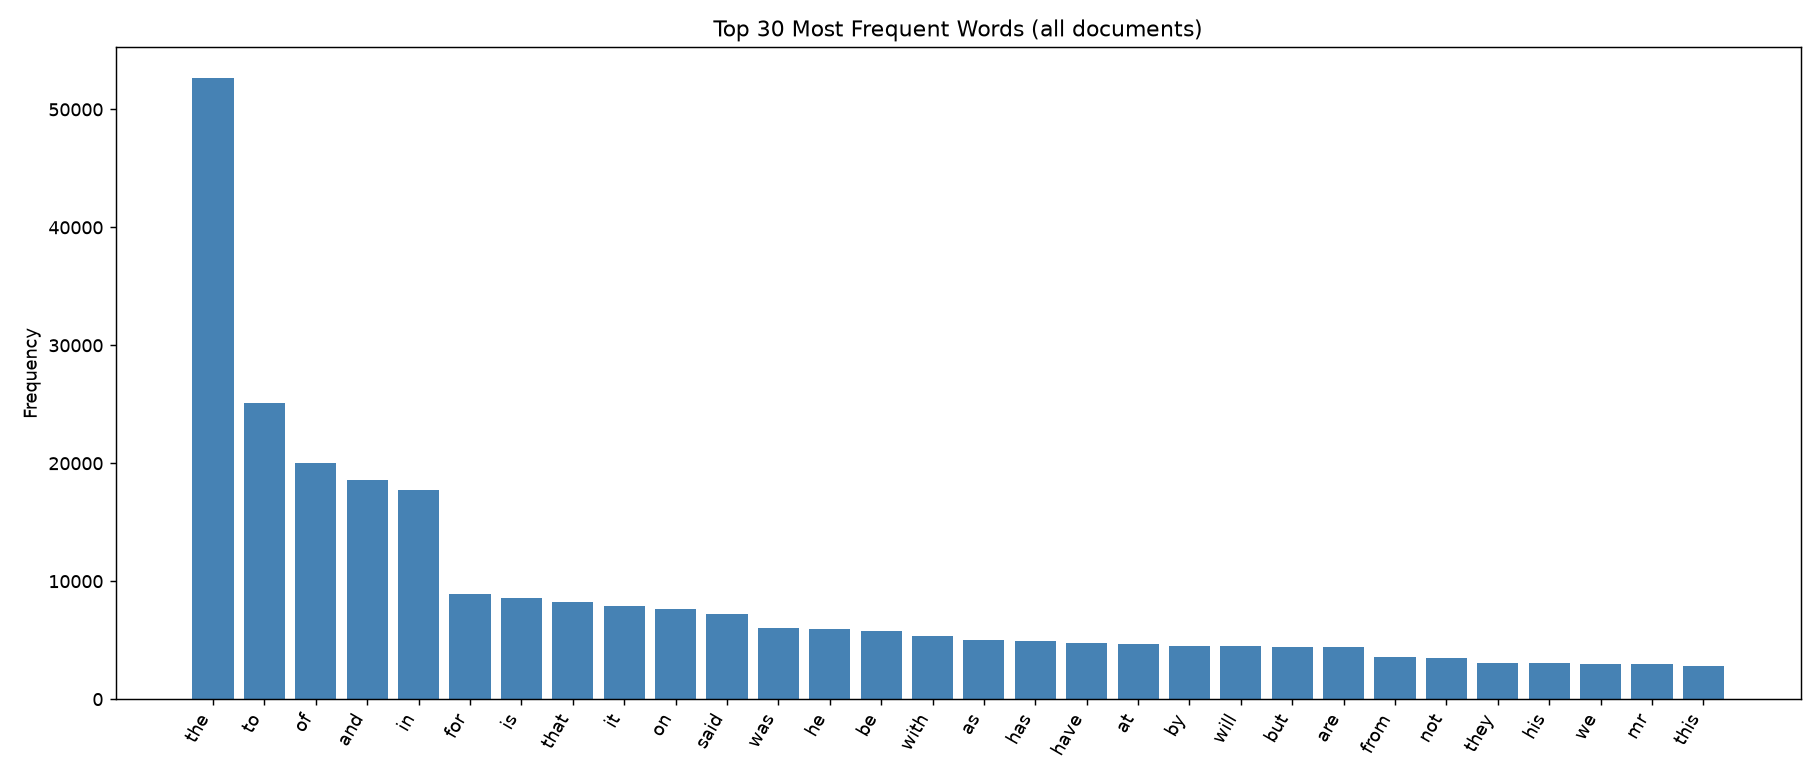
\includegraphics[width=0.95\textwidth]{q8_top30_wo_stopwords.png}
        \caption{۳۰ کلمه پرتکرار بدون حذف کلمات توقف (غلبه کامل حروف ربط و اضافه)}
        \label{fig:top30_no_stop}
    \end{figure}

   
    \begin{figure}[h!]
        \centering
        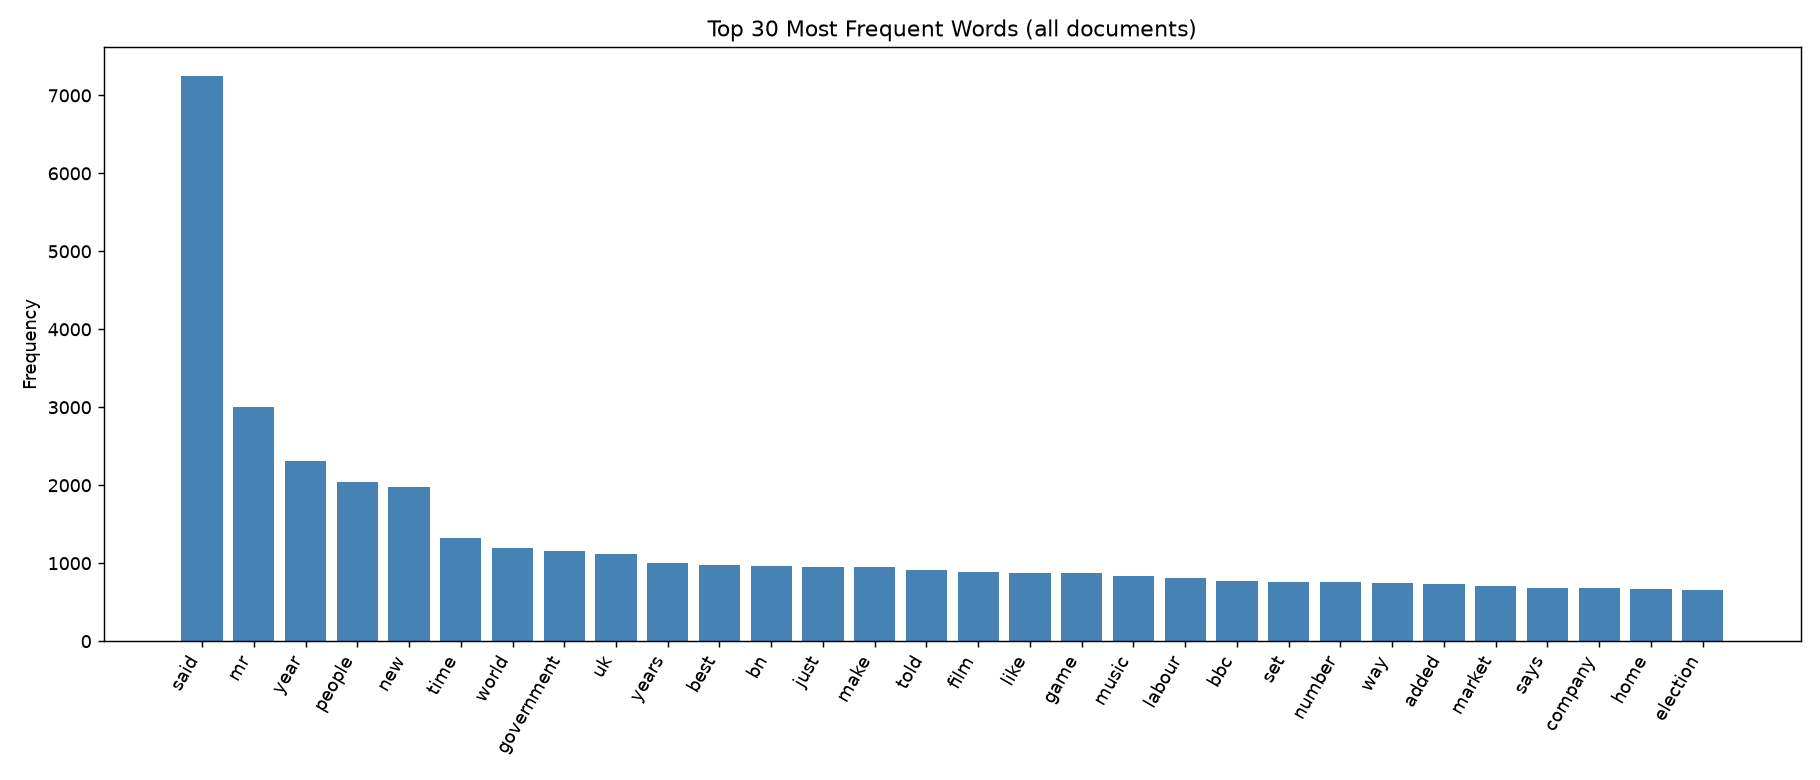
\includegraphics[width=0.95\textwidth]{q8_top30_w_stopwords.png}
        \caption{۳۰ کلمه پرتکرار پس از حذف کلمات توقف (نمایان شدن کلمات کلیدی موضوعی)}
        \label{fig:top30_with_stop}
    \end{figure}

    \begin{itemize}
        \item \textbf{تحلیل حالت اول (بدون حذف کلمات توقف --- شکل \ref{fig:top30_no_stop}):} 
        همان‌طور که در نمودار اول مشاهده می‌شود، کلماتی مانند \lr{``the''} (با بیش از ۵۰,۰۰۰ تکرار)، \lr{``to''}، \lr{``of''} و \lr{``and''} کاملاً بر داده‌ها غلبه کرده‌اند. این کلمات صرفاً نقش ساختاری در زبان انگلیسی دارند و کوچک‌ترین اطلاعاتی درباره موضوع اصلی سند (مانند ورزشی، سیاسی یا علمی بودن آن) به ما نمی‌دهند.
        
        \item \textbf{تحلیل حالت دوم (با حذف کلمات توقف --- شکل \ref{fig:top30_with_stop}):} 
        در نمودار دوم، با فعال‌سازی پارامتر \lr{\texttt{stopwords=True}} و فیلتر کردن این کلمات بیهوده، سقف فرکانس کلمات به زیر ۸,۰۰۰ تکرار کاهش یافته است. با حذف نویزهای زبانی، کلمات معنادار و موضوعی تری مانند \lr{``government''} (دولت)، \lr{``film''} (فیلم)، \lr{``game''} (بازی)، \lr{``music''} (موسیقی) و \lr{``election''} (انتخابات) ظاهر شده‌اند که به ما در دسته‌بندی و تحلیل محتوایی اسناد کمک شایانی می‌کنند.
    \end{itemize}

\noindent\textbf{سوال ۹ --- رسم ابر کلمات اختصاصی براساس وزن‌دهی \lr{TF-IDF}}
    
   \noindent در این بخش، هدف نمایش بصری کلمات کلیدی اسناد با استفاده از یک ابر کلمات (\lr{Word Cloud}) اختصاصی است. از آن‌جایی که پکیج پیش‌فرض \lr{\texttt{wordcloud}} در حالت آفلاین در دسترس نبوده، پیاده‌سازی به صورت دستی و با استفاده از توانمندی‌های ترسیم کتابخانه‌ی \lr{\texttt{matplotlib}} انجام گرفته است. معیار انتخاب کلمات، وزن مجموع فرکانس سند معکوس (\lr{TF-IDF}) آن‌هاست. کد بهینه‌شده به صورت زیر است:

\begin{latin}
\begin{lstlisting}[language=Python]
# ============================================================
# Q9 — Word cloud (top 20 words by TF-IDF), custom-rendered
# (wordcloud package unavailable offline -> manual matplotlib rendering)
# ============================================================
def q9_wordcloud(df, fname):
    extra_stop = ['said', 'mr', 'told', 'year', 'years', 'new', 'time', 'best', 'world']
    stop_words = list(ENGLISH_STOP_WORDS.union(extra_stop))

    vectorizer = TfidfVectorizer(stop_words=stop_words, max_df=0.9, min_df=2)
    tfidf = vectorizer.fit_transform(df['clean_text'])
    scores = np.asarray(tfidf.sum(axis=0)).ravel()
    vocab = vectorizer.get_feature_names_out()

    top_idx = np.argsort(scores)[::-1][:20]
    top_words = [(vocab[i], scores[i]) for i in top_idx]

    random.seed(7)
    fig, ax = plt.subplots(figsize=(12, 8))
    ax.axis('off')
    
    max_score = max(s for _, s in top_words)
    min_score = min(s for _, s in top_words)
    placed = []

    def overlaps(x, y, w, h, placed):
        for (px, py, pw, ph) in placed:
            if abs(x - px) < (w + pw) / 2 * 0.75 and abs(y - py) < (h + ph) / 2 * 0.75:
                return True
        return False

    for word, score in top_words:
        size = 16 + 55 * (score - min_score) / (max_score - min_score)
        
        for _ in range(300):
            x = random.uniform(0.1, 0.9)
            y = random.uniform(0.1, 0.9)
            w = len(word) * size * 0.011
            h = size * 0.02
            if not overlaps(x, y, w, h, placed):
                placed.append((x, y, w, h))
                break
        
        color = plt.cm.tab20(random.random())
        ax.text(x, y, word, fontsize=size, ha='center', va='center', color=color,
                fontweight='bold', fontfamily='sans-serif', transform=ax.transAxes)

    ax.set_title('Top 20 Words Wordcloud', fontsize=16)
    plt.tight_layout()
    % plt.savefig(f'media/{fname}.png', dpi=130)
    plt.close(fig)
    
    return top_words
\end{lstlisting}
\end{latin}

    \subsection*{توضیح عملکرد متدها و تغییرات جدید:}

    \paragraph{۱. توسعه‌ی کلمات توقف (\texttt{stop\_words}):}\hspace{-10pt}
    مجموعه‌ای از کلمات عمومی انگلیسی (\lr{\texttt{ENGLISH\_STOP\_WORDS}}) با کلمات پر تکرار کم‌اهمیت دیگر که در متغیر \lr{\texttt{extra\_stop}} تعریف شده‌اند، ادغام (\lr{\texttt{union}}) می‌شوند. این کار باعث تفکیک کلمات موضوعی باارزش از کلمات تکراری زبان می‌شود.

    \paragraph{۲. بردارسازی با معیار \lr{TF-IDF} (\texttt{TfidfVectorizer}):}\hspace{-10pt}
    یک مدل بردارساز با حذف کلمات توقف تعریف می‌شود. پارامتر \lr{\texttt{max\_df=0.9}} کلماتی را که در بیش از ۹۰ درصد اسناد تکرار شده‌اند حذف می‌کند و \lr{\texttt{min\_df=2}} کلماتی را که کمتر از ۲ بار در کل پیکره متنی تکرار شده‌اند نادیده می‌گیرد. در نهایت، با متد \lr{\texttt{fit\_transform()}} ماتریس ویژگی‌های اسناد محاسبه می‌شود.

    \paragraph{۳. استخراج کلمات کلیدی برتر براساس مجموع امتیازها:}\hspace{-10pt}
    با محاسبه‌ی مجموع امتیازات ماتریس در طول ستون‌ها (\lr{\texttt{tfidf.sum(axis=0)}}) و مرتب‌سازی نزولی اندیس‌ها با استفاده از \lr{\texttt{np.argsort}}، ۲۰ کلمه‌ی برتر که بیشترین وزنِ مجموع را در کل پیکره متنی دارند استخراج می‌شوند.

    \paragraph{۴. الگوریتم چیدمان غیرهم‌پوشان (\texttt{overlaps}):}\hspace{-10pt}
    برای جلوگیری از هم‌پوشانی و روی هم افتادن کلمات در تصویر خروجی، تابع کمکی \lr{\texttt{overlaps}} تعریف شده است. این تابع با تخمین زدن کادر پیرامونی هر کلمه بر اساس طول کلمه و ابعاد فونت، فاصله‌ی موقعیت کلمه‌ی جدید با کلماتی که پیش‌تر جایگذاری شده‌اند را بررسی کرده و در صورت تداخل، موقعیت تصادفی جدیدی را امتحان می‌کند.

    \paragraph{۵. شبیه‌سازی ابر کلمات و بهبودهای بصری جدید:}\hspace{-10pt}
    \begin{itemize}
        \item \textbf{مقیاس‌دهی پویا به فونت کلمات:} اندازه‌ی قلم (\lr{\texttt{size}}) هر کلمه متناسب با فرمول نگاشت خطی بین بازه‌ی ۱۶ الی ۷۱ پیکسل بر اساس امتیاز \lr{TF-IDF} آن تعیین می‌شود تا کلمات با ارزش‌تر، بزرگ‌تر رندر شوند.
        \item \textbf{رنگ‌آمیزی با پالت متمایز \lr{\texttt{tab20}}:} رنگ هر کلمه به طور تصادفی از پالت رنگی استاندارد و متمایز \lr{\texttt{tab20}} تخصیص می‌یابد تا کنتراست و خوانایی کلمات افزایش یابد.
        \item \textbf{بهبود فونت و چیدمان:} فونت نوشته‌ها به حالت بدون سریف (\lr{\texttt{sans-serif}}) و ضخیم (\lr{\texttt{bold}}) تغییر کرده است.
        \item \textbf{ذخیره‌سازی پویا:} تصویر نهایی با قالب پویای نام فایل خروجی (\lr{\texttt{fname}}) در مسیر \lr{\texttt{media/}} آماده‌ی ذخیره‌سازی است.
    \end{itemize}

    \paragraph{۶. تحلیل بصری و بررسی خروجی ابر کلمات جدید:}\hspace{-10pt}
    تصویر زیر خروجی نهایی حاصل از اجرای تابع بر روی ۲۰ کلمه‌ی برتر با معیار وزن‌دهی \lr{TF-IDF} را با پالت رنگی متمایز نشان می‌دهد:

    \begin{figure}[h!]
        \centering
        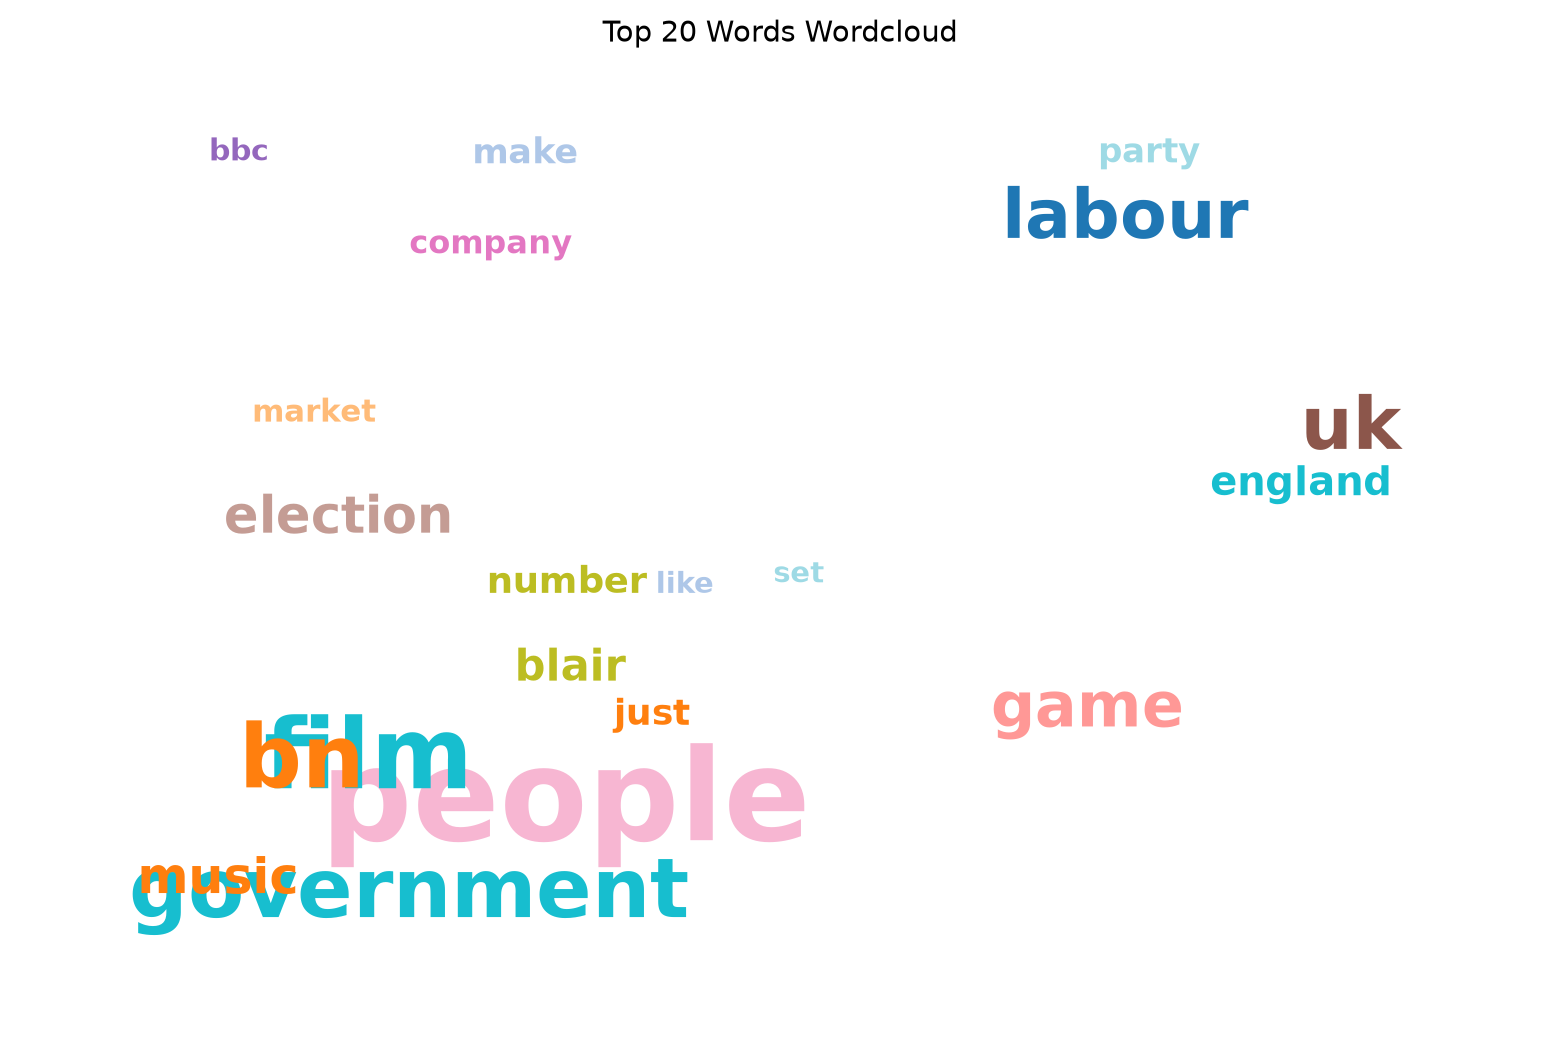
\includegraphics[width=0.9\textwidth]{q9_wordcloud.png}
        \caption{ابر کلمات اختصاصی رسم‌شده برای ۲۰ کلمه برتر بر اساس امتیاز مجموع TF-IDF}
        \label{fig:q9_wordcloud_2}
    \end{figure}

    \begin{itemize}
        \item \textbf{ابعاد بصری و وزن‌دهی معنایی کلمات:}
        همان‌طور که در شکل \ref{fig:q9_wordcloud_2} مشخص است، کلماتی نظیر \lr{``people''} (به رنگ صورتی)، \lr{``government''} (به رنگ فیروزه‌ای)، \lr{``labour''} (به رنگ آبی تیره) و \lr{``film''} با فونت بسیار بزرگ‌تری رندر شده‌اند. این اندازه بزرگ نشان‌دهنده‌ی امتیاز بالا و مجموع وزن \lr{TF-IDF} بالای آن‌ها در اسناد است. یعنی این واژه‌ها نه‌تنها تکرار قابل‌قبولی دارند، بلکه به شدت متمایزکننده‌ی موضوعات اصلی (مانند سیاست، سینما و اقتصاد) هستند.
        
        \item \textbf{تمایز موضوعی آشکار:}
        برخلاف نمودارهای فرکانس ساده، در این تصویر کلماتی مانند \lr{``election''} (انتخابات)، \lr{``blair''} (بلر - نخست‌وزیر سابق بریتانیا)، \lr{``game''} (بازی)، \lr{``market''} (بازار)، \lr{``music''} (موسیقی) و \lr{``company''} (شرکت) به وضوح دیده می‌شوند. این توزیع کلمات نشان می‌دهد که پیکره متنی ما به طور مشخص شامل موضوعاتی پیرامون سیاست بریتانیا، اخبار بازار و تجارت، دنیای سرگرمی (موسیقی/بازی/فیلم) و تکنولوژی است.
        
        \item \textbf{تأیید کارکرد فیلترهای بالاگذر و پایین‌گذر:}
        موفقیت الگوریتم در این است که کلمات بسیار عمومی مانند \lr{``year''}، \lr{``new''} یا کلمات توقف انگلیسی استاندارد که پیش‌تر در واژه‌نامه‌ی \lr{\texttt{stop\_words}} قرار گرفتند، به کلی فیلتر شده‌اند و در ابر کلمات حضور ندارند. این فرآیند بستری عالی و با کیفیت را برای مرحله‌ی بعدی یعنی ساخت ماتریس برداری اسناد ایجاد می‌کند.
    \end{itemize}

\noindent\textbf{سوال ۱۰ --- ساخت ماتریس کیسه کلمات (BoW) با واژگان سفارشی و تقسیم‌بندی داده‌ها}
    
   \noindent در این مرحله، هدف ساخت ماتریس کیسه کلمات (\lr{Bag-of-Words}) با استفاده از یک واژگان مشخص واژه‌نامه است که از فایل خارجی \lr{\texttt{words.csv}} بارگذاری می‌شود. در نهایت داده‌ها به دو بخشِ مجموعه‌ی کاری (آموزش) و مجموعه‌ی آزمون نگهداشت تقسیم می‌شوند. کد مربوطه به صورت زیر است:

\begin{latin}
\begin{lstlisting}[language=Python]
# ============================================================
# Q10 — Bag-of-Words matrix using words.csv vocabulary
# ============================================================
def q10_bow_matrix(df):
    words_df = pd.read_csv('words.csv', header=None)    
    vocabulary_list = words_df[0].astype(str).str.lower().tolist()
    
    vectorizer = CountVectorizer(vocabulary=vocabulary_list)
    bow = vectorizer.fit_transform(df['clean_text'])
    bow_matrix = bow.toarray()
    
    print(f"\nQ10 | BoW matrix shape: {bow_matrix.shape}  (docs x |vocab|={len(vocabulary_list)})")
    
    return bow_matrix


def split_2000_225(df, bow_matrix):
    """Split literally: first 2000 rows = working set, last 225 = held-out test."""
    df_train = df.iloc[:2000].reset_index(drop=True)
    df_test = df.iloc[2000:].reset_index(drop=True)
    bow_train = bow_matrix[:2000]
    bow_test = bow_matrix[2000:]
    print("Split | train:", df_train.shape, bow_train.shape,
          "| test:", df_test.shape, bow_test.shape)
    print("Split | NOTE: dataset is label-sorted, so the literal last-225 test rows "
          "are ALL label 4 (Business). See shuffled version in Q20 for a fair "
          "per-category evaluation.")
    return df_train, df_test, bow_train, bow_test
\end{lstlisting}
\end{latin}

    \subsection*{توضیح عملکرد متدها و تغییرات جدید:}

    \paragraph{۱. بارگذاری و آماده‌سازی پویا واژگان (Vocabulary) :}
    \begin{itemize}
        \item \textbf{( one header ،’ ’words.csv ) pd.read\_csv= }: واژه‌های مرجع مستقیماً از فایل \lr{\texttt{words.csv}} بارگذاری می‌شوند. از آنجا که این فایل فاقد ردیف هدر (عنوان ستون) است، پارامتر \lr{\texttt{header=None}} تنظیم شده است.
        \item \textbf{یکدست‌سازی واژگان (\texttt{vocabulary\_list})}: با دستور \lr{\texttt{astype(str).str.lower().tolist()}}، تمامی کلمات موجود در ستون اول فایل به نوع رشته تبدیل شده، حروف آن‌ها کوچک می‌شود و در نهایت به یک لیست معمولی پایتون تبدیل می‌گردند. این کار باعث تطابق کامل و بدون خطای واژگان با متون پیش‌پردازش‌شده می‌شود.
    \end{itemize}

    \paragraph{۲. ساخت ماتریس کیسه کلمات (\texttt{CountVectorizer}):}
    \begin{itemize}
        \item \textbf{محدودسازی ستون‌ها به واژگان سفارشی}: با پاس دادن \lr{\texttt{vocabulary=vocabulary\_list}} به کلاس \lr{\texttt{CountVectorizer}}، مدل را موظف می‌کنیم که ماتریس را صرفاً بر اساس کلمات این لیست بسازد. هر کلمه‌ای در اسناد که در این لیست نباشد، نادیده گرفته خواهد شد.
        \item \textbf{تبدیل به آرایه متراکم (\texttt{toarray()})}: خروجی متد \lr{\texttt{fit\_transform}} یک ماتریس خلوت است که برای انجام راحت‌تر محاسبات جبر خطی بعدی (مانند تجزیه مقادیر منفرد) با متد \lr{\texttt{toarray()}} به یک آرایه دو بعدی استاندارد و متراکم \lr{NumPy} تبدیل می‌شود. ابعاد این ماتریس برابر با $2225 \times M$ خواهد بود که در آن $M$ تعداد کلمات واژه‌نامه است.
    \end{itemize}

    \paragraph{۳. تقسیم‌بندی داده‌ها به مجموعه‌های آموزش و آزمون:}\hspace{-10pt}
    تابع \lr{\texttt{split\_2000\_225}} داده‌های ورودی را به دو بخش افقی تقسیم می‌کند:
    \begin{itemize}
        \item \textbf{مجموعه آموزش (\texttt{train})}: شامل ۲۰۰۰ سطر اول اسناد و بردارهای کیسه کلمات متناظر با آن‌هاست.
        \item \textbf{مجموعه آزمون (\texttt{test})}: شامل ۲۲۵ سطر پایانی به عنوان داده‌های آزمون مجزا و دست‌نخورده است.
        \item \textbf{نکته مهم توزیع دسته‌ها}: به دلیل مرتب بودن اولیه مجموعه داده بر اساس برچسب‌ها، ۲۲۵ سطر پایانی همگی دارای برچسب شماره ۴ (تجارت) هستند. این تقسیم‌بندی صِرفاً یک پیاده‌سازی گام‌به‌گام اولیه است و جابجایی تصادفی داده‌ها (\lr{Shuffle}) در بخش‌های بعدی برای ارزیابی نهایی به کار گرفته خواهد شد.
    \end{itemize}

\paragraph{۴. خروجی فرآیند بردارسازی و تحلیل ساختار ماتریس \lr{BoW}:}\hspace{-10pt}
    پس از اجرای تابع، آرایه خروجی و ابعاد به دست آمده به شکل زیر نمایش داده می‌شود:

    \begin{figure}[h!]
        \centering
        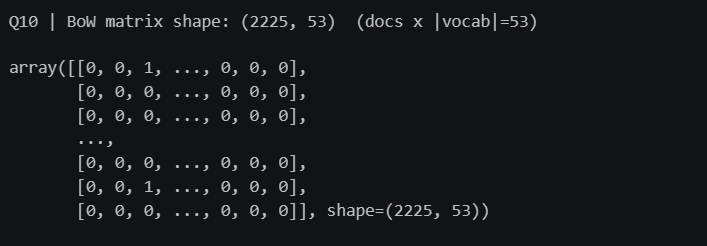
\includegraphics[width=0.85\textwidth]{Output10.png}
        \caption{نمای کلی از ماتریس فرکانسی کیسه کلمات (BoW) و ابعاد آن در خروجی مفسر}
        \label{fig:q10_bow_output}
    \end{figure}

    \begin{itemize}
        \item \textbf{بررسی ابعاد ماتریس (\lr{shape=(2225, 53)}):} 
        خروجی نشان می‌دهد که ماتریس حاصل دارای ۲۲۲۵ سطر (تعداد کل اسناد) و ۵۳ ستون است. این ابعاد دقیقاً تایید می‌کند که تعداد واژه‌های استخراج‌شده از فایل \lr{\texttt{words.csv}} برابر با ۵۳ کلمه کلیدی متمایز بوده است. بنابراین هر سند متنی به یک بردار ویژگی ۵۳ بُعدی تصویر می‌شود.
        
        \item \textbf{تحلیل ساختار عددی ماتریس خلوت (\lr{Sparse Matrix}):} 
        همان‌طور که در آرایه‌ی خروجی شکل \ref{fig:q10_bow_output} مشهود است، بخش زیادی از درایه‌های ماتریس مقدار صفر ($0$) دارند. این ویژگی به دلیل ماهیت اسناد متنی است؛ چرا که در هر سند متنی کوتاه، تنها تعداد انگشت‌شماری از واژگان ۵۳گانه استفاده شده‌اند. حضور مقادیری مانند $1$ در درایه‌ها نمایانگر دفعات تکرار آن واژه‌ی خاص از واژه‌نامه در سند متناظر است. این ساختار صفر و یک فرکانسی، پایه‌ی ریاضی مراحل بعدی تحلیل‌های جبر خطی پروژه را شکل می‌دهد.
    \end{itemize}

\noindent    \textbf{بخش افراز مجموعه داده ( Dataset Partitioning ) --- تقسیم ساده در مقابل تقسیم تصادفی}
    
  \noindent  در این بخش، هدف تقسیم مجموعه داده به دو بخش آموزش (\lr{Train}) با ابعاد ۲۰۰۰ نمونه و آزمون (\lr{Test}) با ابعاد ۲۲۵ نمونه است. برای این کار دو تابع با رویکردهای متفاوت پیاده‌سازی شده است که کد آن‌ها به صورت زیر است:

\begin{latin}
\begin{lstlisting}[language=Python]
# ============================================================
# Dataset Partitioning (Simple vs Shuffled Split)
# ============================================================
def split_2000_225(df, bow_matrix):
    """Split literally: first 2000 rows = working set, last 225 = held-out test."""
    df_train = df.iloc[:2000].reset_index(drop=True)
    df_test = df.iloc[2000:].reset_index(drop=True)
    bow_train = bow_matrix[:2000]
    bow_test = bow_matrix[2000:]
    print("Split | train:", df_train.shape, bow_train.shape,
          "| test:", df_test.shape, bow_test.shape)
    return df_train, df_test, bow_train, bow_test

def split_2000_225_shuffle(df, bow_matrix):
    df_train, df_test, bow_train, bow_test = train_test_split(
        df,
        bow_matrix,
        train_size=2000,
        shuffle=True,
        random_state=42
    )
    
    df_train = df_train.reset_index(drop=True)
    df_test = df_test.reset_index(drop=True)
    
    print("Split | train:", df_train.shape, bow_train.shape,
          "| test:", df_test.shape, bow_test.shape)
    return df_train, df_test, bow_train, bow_test
\end{lstlisting}
\end{latin}

    \subsection*{توضیح عملکرد و مقایسه متدها:}

    \paragraph{۱. تابع تقسیم ترتیبی و ساده (\texttt{split\_2000\_225}):}
    \begin{itemize}
        \item \textbf{عملکرد:} این تابع با استفاده از برش‌زدن ساده ایندکس‌ها (\lr{Slicing}) با دستور \lr{\texttt{.iloc}}، دقیقا ۲۰۰۰ سطر نخست را به عنوان مجموعه آموزش و ۲۲۵ سطر انتهایی را به عنوان مجموعه آزمون جدا می‌کند. 
        \item \textbf{ریست کردن ایندکس:} با متد \lr{\texttt{reset\_index(drop=True)}} ایندکس‌های دیتافریم‌های جدید دوباره از صفر مقداردهی می‌شوند تا در تحلیل‌های بعدی خطایی رخ ندهد.
        \item \textbf{اشکال ساختاری (اریب بودن داده‌ها):} از آن‌جا که داده‌های اولیه بر اساس برچسب‌ها مرتب شده‌اند، ۲۲۵ سطر آخر همگی متعلق به کلاس شماره ۴ (\lr{Business}) خواهند بود. این یعنی مدل هیچ داده‌ی ارزیابی از دسته‌های دیگر (مانند سیاست یا ورزش) در این نوع تقسیم‌بندی نخواهد داشت که منجر به ارزیابی غیرمنصفانه می‌شود.
    \end{itemize}

    \paragraph{۲. تابع تقسیم تصادفی مجهز به برهم‌زدن (\texttt{split\_2000\_225\_shuffle}):}
    \begin{itemize}
        \item \textbf{عملکرد:} این تابع از متد استاندارد \lr{\texttt{train\_test\_split}} استفاده می‌کند تا فرآیند تقسیم‌بندی را به شکل کاملاً علمی و توزیع‌شده انجام دهد.
        \item \textbf{پارامتر \texttt{shuffle=True}:} قبل از جدا کردن سطرها، موقعیت تمامی نمونه‌ها به صورت تصادفی برهم زده می‌شود. این کار تضمین می‌کند که داده‌های هر دو بخش آموزش و آزمون شامل توزیع یکنواختی از تمامی کلاس‌ها (سیاست، تجارت، ورزش و غیره) باشند.
        \item \textbf{پارامتر \texttt{random\_state=42}:} با تعیین هسته تصادفی ثابت (عدد ۴۲)، فرآیند مخلوط‌سازی داده‌ها در هر بار اجرای کد دقیقاً یکسان خواهد بود تا نتایج آزمایش‌ها قابل بازتولید (\lr{Reproducible}) باشد.
    \end{itemize}

\noindent\textbf{سوال ۱۱ --- استانداردسازی داده‌ها و اعمال تجزیه مقادیر منفرد (SVD)}
    
  \noindent  در این بخش، ابتدا داده‌های فرکانسی کیسه کلمات (\lr{BoW}) مقیاس‌دهی و استانداردسازی می‌شوند تا اثر تفاوت در طول اسناد و فرکانس‌های مطلق واژه‌ها خنثی شود. سپس، با استفاده از الگوریتم تجزیه مقادیر منفرد (\lr{SVD})، ماتریس داده‌ها به مؤلفه‌های سازنده‌اش تجزیه می‌گردد. کد این بخش به صورت زیر است:

\begin{latin}
\begin{lstlisting}[language=Python]
# ============================================================
# Q11 — Standardization and Singular Value Decomposition (SVD)
# ============================================================
def q11_standardize_and_svd(bow_matrix):
    scaler = StandardScaler()
    bow_scaled = scaler.fit_transform(bow_matrix)
    
    U, S, Vt = np.linalg.svd(bow_scaled, full_matrices=False)
    
    print("=== SVD Matrices Dimensions ===")
    print(f"Original Scaled Matrix (M x N) : {bow_scaled.shape}")
    print(f"U Matrix (Left Singular)       : {U.shape}")
    print(f"S Array (Singular Values)      : {S.shape}")
    print(f"V^T Matrix (Right Singular)    : {Vt.shape}")
    
    return bow_scaled, U, S, Vt
\end{lstlisting}
\end{latin}

    \subsection*{توضیح عملکرد متدها و مفاهیم ریاضی:}

    \paragraph{۱. استانداردسازی با \texttt{StandardScaler}:}\hspace{-10pt}
    از آن‌جا که کلمات مختلف فرکانس‌های متفاوتی دارند، واژه‌های بسیار پرتکرار می‌توانند به طور ناعادلانه‌ای روی محاسبات فاصله و ابعاد اثر بگذارند. کلاس \lr{\texttt{StandardScaler}} با کسر میانگین هر ویژگی (ستون) و تقسیم آن بر انحراف معیار، داده‌ها را به گونه‌ای مقیاس‌دهی می‌کند که میانگین آن‌ها برابر با $0$ و واریانس آن‌ها برابر با $1$ شود:
    $$x_{\text{scaled}} = \frac{x - \mu}{\sigma}$$

    \paragraph{۲. تجزیه مقادیر منفرد (SVD) به فرم باریک (\texttt{full\_matrices=False}):}\hspace{-10pt}
    رابطه ریاضی حاکم بر این تجزیه به صورت زیر است:
    $$A_{M \times N} = U_{M \times K} \Sigma_{K \times K} V^T_{K \times N}$$
    که در آن $K = \min(M, N)$ است. 
    \begin{itemize}
        \item تنظیم پارامتر \lr{\texttt{full\_matrices=False}} فرمت کاهش‌یافته یا باریک (\lr{Reduced/Thin SVD}) را پیاده‌سازی می‌کند. این کار به جای تولید ماتریس‌های مربعی بزرگ و غیرضروری، ابعاد مؤلفه‌ها را محدود به کوچک‌ترین بعد ماتریس اصلی ($N$ یا همان ۵۳ بعد واژگان) نگه می‌دارد تا از هدررفت حافظه و محاسبات اضافه جلوگیری شود.
    \end{itemize}

    \paragraph{۳. تحلیل ابعاد ماتریس‌های خروجی در ترمینال:}\hspace{-10pt}
    با فرض اعمال این تابع روی کل مجموعه داده با ابعاد $2225 \times 53$، ابعاد ماتریس‌ها در خروجی به شرح زیر تحلیل می‌شوند:
    \begin{itemize}
        \item \textbf{ماتریس استاندارد شده (\lr{\texttt{bow\_scaled}}):} ابعاد آن دست‌نخورده و برابر با $(2225, 53)$ باقی می‌ماند.
        \item \textbf{ماتریس بردار‌های منفرد چپ (\lr{\texttt{U}}):} ابعاد آن $(2225, 53)$ خواهد بود که اسناد را در فضای پنهان (\lr{Latent Space}) توصیف می‌کند.
        \item \textbf{آرایه مقادیر منفرد (\lr{\texttt{S}}):} این آرایه تک‌بعدی شامل ۵۳ مقدار منفرد مرتب‌شده به صورت نزولی است که نشان‌دهنده میزان پراکندگی یا اهمیت هر یک از محورهای مختصات جدید است.
        \item \textbf{ماتریس بردار‌های منفرد راست (\lr{\texttt{Vt}}):} ابعاد آن $(53, 53)$ خواهد بود که کلمات را در فضای پنهان توصیف کرده و ارتباط واژگان با ویژگی‌های پنهان را مشخص می‌کند.
    \end{itemize}

    \paragraph{۴. خروجی فرآیند تجزیه SVD و تحلیل ابعاد ماتریس‌ها:}
    پس از اجرای تابع بر روی داده‌های استاندارد شده مجموعه آموزش (که شامل ۲۰۰۰ سند است)، ابعاد واقعی ماتریس‌های حاصل به شکل زیر در خروجی ظاهر می‌شود:

    \begin{figure}[h!]
        \centering
        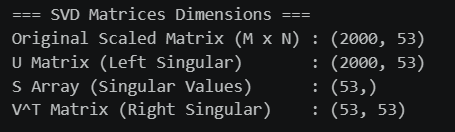
\includegraphics[width=0.85\textwidth]{Output11.png}
        \caption{ابعاد چاپ‌شده برای ماتریس‌های تجزیه SVD در خروجی محیط پایتون}
        \label{fig:q11_svd_output}
    \end{figure}

    \begin{itemize}
        \item \textbf{ماتریس مقیاس‌شده اصلی (\lr{Original Scaled Matrix}):} 
        ابعاد این ماتریس برابر با $(2000, 53)$ است. این نشان می‌دهد که تجزیه بر روی بخش آموزش داده‌ها (با ۲۰۰۰ سند و ۵۳ ویژگی کلیدی) اعمال شده است.
        
        \item \textbf{ماتریس $U$ (بردار‌های منفرد چپ):} 
        ابعاد این ماتریس برابر با $(2000, 53)$ است. به دلیل تنظیم حالت باریک (\lr{\texttt{full\_matrices=False}})، تعداد ستون‌های این ماتریس به جای ۲۰۰۰ (در حالت $SVD$ کامل)، برابر با تعداد کلمات واژه‌نامه (یعنی ۵۳) محدود شده است که هر سند را در فضای ویژگی‌های پنهان جدید نمایش می‌دهد.
        
        \item \textbf{آرایه $S$ (مقادیر منفرد):} 
        ابعاد این آرایه به صورت تک‌بعدی با طول ۵۳ رندر شده است (\lr{\texttt{(53,)}}). این ۵۳ مقدار مثبت و نزولی، میزان واریانس و پراکندگی داده‌ها را روی تک‌تک مولفه‌های جدید نشان می‌دهند.
        
        \item \textbf{ماتریس $V^T$ (بردار‌های منفرد راست):} 
        ابعاد آن $(53, 53)$ است که ارتباط مستقیم بین ۵۳ کلمه‌ی واژه‌نامه اصلی و ۵۳ بعد پنهان جدید کشف‌شده توسط الگوریتم را فرموله‌سازی می‌کند.
    \end{itemize}
\newpage

\noindent\textbf{سوال ۱۲ --- تعیین پویای آستانه حفظ اطلاعات، ترسیم نمودار و اعمال \lr{Truncated SVD}}
    
\noindent در این گام، هدف تعیین ساختاریافته و خودکار بعد بهینه ($k$) برای کاهش بعد داده‌ها است. به جای حدس شهودی، بعد بهینه دقیقاً بر اساس آستانه‌ی ریاضی حفظ ۹۰ درصد واریانس کل داده‌ها محاسبه می‌شود. کد بهینه‌شده به صورت زیر است:

\begin{latin}
\begin{lstlisting}[language=Python]
# ============================================================
# Q12 — Scree plot + threshold selection + Truncated SVD + error
# ============================================================
def q12_truncated_svd(bow_scaled, U, S, Vt, fname, fname2, variance_threshold=0.90):
    total_variance = np.sum(S ** 2)
    cumulative_variance = np.cumsum(S ** 2) / total_variance
    
    k_optimal = np.argmax(cumulative_variance >= variance_threshold) + 1
    
    fig, ax = plt.subplots(figsize=(10, 6))

    ax.plot(cumulative_variance, color='steelblue', linewidth=2)
    ax.axhline(y=variance_threshold, color='red', linestyle='--', label=f'Threshold ({variance_threshold*100}%)')
    ax.axvline(x=k_optimal, color='green', linestyle='--', label=f'Optimal k = {k_optimal}')
    
    ax.set_title('Cumulative Explained Variance by Singular Values', fontsize=14)
    ax.set_xlabel('Number of Singular Values (k)', fontsize=12)
    ax.set_ylabel('Cumulative Variance', fontsize=12)
    ax.legend(loc='lower right')
    plt.grid(True, alpha=0.3)
    plt.tight_layout()
    plt.savefig(f'media/{fname}', dpi=130)
    plt.close(fig)    

    print(f"Suggested k to retain {variance_threshold*100}% variance: {k_optimal}")
    
    U_truncated = U[:, :k_optimal]
    S_truncated = np.diag(S[:k_optimal])
    Vt_truncated = Vt[:k_optimal, :]
    
    print("\n=== Truncated Matrices Dimensions ===")
    print(f"U_k shape  : {U_truncated.shape}")
    print(f"S_k shape  : {S_truncated.shape}")
    print(f"Vt_k shape : {Vt_truncated.shape}")
    
    bow_reconstructed = np.dot(U_truncated, np.dot(S_truncated, Vt_truncated))
    
    reconstruction_error = np.linalg.norm(bow_scaled - bow_reconstructed, 'fro')
    print(f"Reconstruction Error : {reconstruction_error:.4f}")
    
    return U_truncated, S_truncated, Vt_truncated, bow_reconstructed
\end{lstlisting}
\end{latin}

    \subsection*{توضیح عملکرد متدها و منطق ریاضی:}

    \paragraph{۱. محاسبه‌ی واریانس تجمعی توجیه‌شده (\texttt{cumulative\_variance}):}\hspace{-10pt}
    در تجزیه مقادیر منفرد، مجذور هر مقدار منفرد ($s_i^2$) نشان‌دهنده‌ی میزان واریانس (اطلاعات) حفظ‌شده روی آن بعد پنهان است.
    \begin{itemize}
        \item ابتدا کل واریانس با جمع مجذور تمامی مقادیر منفرد محاسبه می‌شود: $\sum s_i^2$.
        \item با تقسیم مجموع تجمعی مجذورات بر واریانس کل، نسبت واریانس تجمعی توجیه‌شده به دست می‌آید که مقداری در بازه‌ی $[0, 1]$ است.
    \end{itemize}

    \paragraph{۲. یافتن خودکار بعد بهینه ($k$):}\hspace{-10pt}
    با دستور \lr{\texttt{np.argmax(cumulative\_variance >= variance\_threshold)}}، نخستین اندیسی که در آن نسبت واریانس تجمعی از آستانه تعریف شده (مثلاً ۹۰٪ یا همان $0.90$) عبور می‌کند به طور خودکار پیدا می‌شود. با اضافه کردن عدد ۱ به این اندیس، مقدار بهینه‌ی $k$ به دست می‌آید.

    \paragraph{۳. رسم تخصصی نمودار تجمعی و خطوط راهنما:}\hspace{-10pt}
    \begin{itemize}
        \item خط افقی نقطه‌چین قرمز رنگ (\lr{red dashed line}) آستانه مورد نیاز (مثلاً ۹۰٪) را روی محور عمودی تصویر می‌کند.
        \item خط عمودی نقطه‌چین سبز رنگ (\lr{green dashed line}) مقدار دقیق $k$ بهینه محاسباتی را روی محور افقی نشان می‌دهد تا نقطه تلاقی آن‌ها کاملاً ملموس باشد.
        \item تصویر نهایی با نام پویا از طریق متغیر \lr{\texttt{fname}} در مسیر مشخص‌شده ذخیره می‌شود.
    \end{itemize}

    \paragraph{۴. کوته‌سازی ماتریس‌ها (\texttt{Truncated SVD}):}\hspace{-10pt}
    پس از تعیین مقدار پویای $k$، ماتریس‌ها بر اساس این بعد جدید برش داده می‌شوند:
    \begin{itemize}
        \item \textbf{\texttt{U\_truncated}}: صرفاً $k$ بعد پنهان برتر برای اسناد نگه داشته می‌شود.
        \item \textbf{\texttt{S\_truncated}}: آرایه مقادیر منفرد برتر به یک ماتریس قطری با ابعاد $k \times k$ تبدیل می‌شود.
        \item \textbf{\texttt{Vt\_truncated}}: صرفاً فرکانس و وزن کلمات روی $k$ بعد پنهان اول حفظ می‌شود.
    \end{itemize}

    \paragraph{۵. بازسازی ماتریس و خطای فروبنیوس:}\hspace{-10pt}
    با ضرب متوالی ماتریس‌های کوته‌سازی‌شده (\lr{\texttt{np.dot}})، ماتریس تقریب‌زده شده با رتبه‌ی پایین ($bow\_reconstructed$) تشکیل می‌شود:
    $$A_k = U_k \cdot \Sigma_k \cdot V^T_k$$
    سپس تفاوت میان ماتریس استاندارد شده‌ی اولیه و ماتریس بازسازی‌شده با استفاده از نرم فروبنیوس (\lr{Frobenius Norm}) به عنوان معیار خطای بازسازی محاسبه می‌گردد. هر چه مقدار $k$ بزرگ‌تر باشد، این خطا به صفر نزدیک‌تر می‌شود، اما بعد فضای ویژگی نیز بزرگ‌تر خواهد شد.

\paragraph{۶. تحلیل تجربی نمودار واریانس تجمعی و تعیین بعد بهینه:}\hspace{-10pt}
    پس از اجرای الگوریتم بر روی داده‌های استاندارد شده‌ی مجموعه آموزش، نمودار تعیین آستانه و فرآیند کاهش بعد به شکل زیر ترسیم و ذخیره می‌شود:

    \begin{figure}[h!]
        \centering
        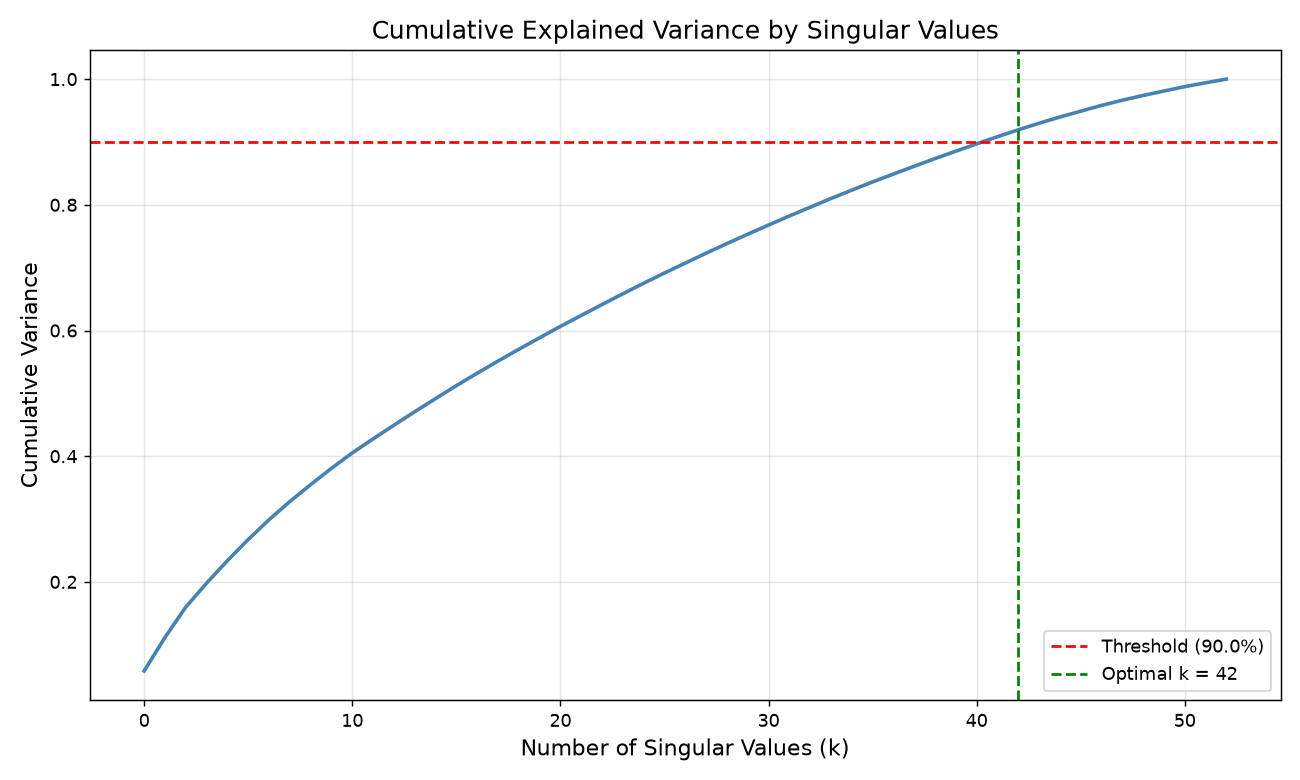
\includegraphics[width=0.9\textwidth]{q12_svd_threshold.png}
        \caption{نمودار واریانس تجمعی توجیه‌شده به همراه خطوط راهنما برای تعیین بعد بهینه $k$}
        \label{fig:q12_svd_threshold}
    \end{figure}

    \begin{itemize}
        \item \textbf{تحلیل منحنی واریانس تجمعی (\lr{Cumulative Variance}):}
        منحنی آبی‌رنگ نشان می‌دهد که با اضافه شدن هر یک از مقادیر منفرد ($k$)، چه میزان از اطلاعات (واریانس) کل داده‌ها پوشش داده می‌شود. شیب صعودی منحنی در ابتدا بسیار تیز است که نشان‌دهنده‌ی تمرکز شدید اطلاعات در مؤلفه‌های پنهان اولیه است. با حرکت به سمت راست، شیب منحنی به تدریج ملایم‌تر می‌شود که رفتاری کاملاً طبیعی در تجزیه مقادیر منفرد است.

        \item \textbf{تعیین بعد بهینه ($k=42$):}
        مبنای تصمیم‌گیری برای کاهش بعد، حفظ حداقل ۹۰ درصد از واریانس کل داده‌ها تعریف شده است:
        \begin{itemize}
            \item خط افقی نقطه‌چین قرمز رنگ (\lr{red dashed line}) مرز بحرانی ۹۰ درصد ($0.90$) را روی محور عمودی مشخص می‌کند.
            \item خط عمودی نقطه‌چین سبز رنگ (\lr{green dashed line}) دقیقاً در نقطه‌ای رسم شده است که منحنی آبی‌رنگ از این مرز عبور می‌کند.
            \item بر اساس محاسبات دقیق کد، در نقطه $k = 42$ میزان واریانس تجمعی توجیه‌شده از ۹۰ درصد فراتر می‌رود. بنابراین، سیستم به طور خودکار بعد فضا را از ۵۳ ویژگی اولیه به ۴۲ مؤلفه پنهان کاهش می‌دهد.
        \end{itemize}

        \item \textbf{نتیجه‌گیری عملی از کاهش بعد:}
        انتخاب $k=42$ نشان می‌دهد که با حذف ۱۱ بعد کم‌اهمیت‌تر (که حدود ۲۰٪ از ابعاد کل واژه‌نامه است)، همچنان بیش از ۹۰٪ از واریانس و اطلاعات ساختاری داده‌ها حفظ می‌شود. این فشرده‌سازی هوشمندانه علاوه بر کاهش حجم محاسبات، با حذف نویزهای موجود در فرکانس‌های ضعیف کلمات، دقت مدل‌های دسته‌بندی بعدی را بهبود می‌بخشد.
    \end{itemize}    
\end{document}